% Section content template for individual Educative lessons
% This file contains the actual content for a specific section
% Generated from Educative API section content

% Section: Requirements for ESPNcricinfo
% Section ID: 5684717988085760
% Section Slug: requirements-for-espncricinfo
% Generated: 2025-12-14T13:32:22.834764

In this lesson, we'll list ESPNcricinfo's requirements. This is a crucial step since requirements define the scope of a problem. Therefore, accurately obtaining and thoroughly understanding them from the interviewer will make the design of the rest of the system smooth and easy.
\\
We'll use the notational convention to identify each requirement with a unique label, ``Rn,'' where ``R'' is short for requirement and ``n'' is a natural number.

\subsection{Requirements collection}\label{CknBwrPXKnOciqLZljpt2}
\\
The requirements for ESPNcricinfo are defined below:

% \vspace{-1.0\baselineskip}
\noindent
\begin{minipage}[t]{0.48\textwidth}\vspace{0pt}
\textbf{R1:} The system shall allow the admin to add or update players, teams, and match statistics.
\\
\textbf{R2:} The system shall enable the commentator to add or modify ball-by-ball commentary, and allow tracking of every score or wicket per ball.
\end{minipage}
\hfill
\begin{minipage}[t]{0.48\textwidth}\vspace{0pt}
\centering

\includegraphics[width=0.5\textwidth]{Images/chapter_26/section_5684717988085760/6663857092427776.png}
\end{minipage}

% \vspace{-1.0\baselineskip}
\noindent
\begin{minipage}[t]{0.48\textwidth}\vspace{0pt}
\textbf{R3:} The system shall support tracking all matches, including Test, ODI, and T20, added or modified by the admin.
\\
\textbf{R4:} The system shall maintain a record of ongoing and historical tournaments and display points tables for all participating teams. The admin is responsible for adding or updating tournaments.
\end{minipage}
\hfill
\begin{minipage}[t]{0.48\textwidth}\vspace{0pt}
\centering

\includegraphics[width=0.5\textwidth]{Images/chapter_26/section_5684717988085760/5507914862428160.png}
\end{minipage}

% \vspace{-1.0\baselineskip}
\noindent
\begin{minipage}[t]{0.48\textwidth}\vspace{0pt}
\textbf{R5:} The system shall display results for all previous matches, including televised ones, by utilizing match data added by the admin.
\\
\textbf{R6:} The system will allow the coach to submit a tournament squad---a group of selected players eligible to participate.
\\
\textbf{R7:} The system shall support playing 11 selections from the tournament squad for each match.
\\
\textbf{R8:} The admin shall be able to manage the entire system by adding or modifying tournaments, matches, teams, players, stadiums, umpires, commentators, and updating stats and news.
\end{minipage}
\hfill
\begin{minipage}[t]{0.48\textwidth}\vspace{0pt}
\centering
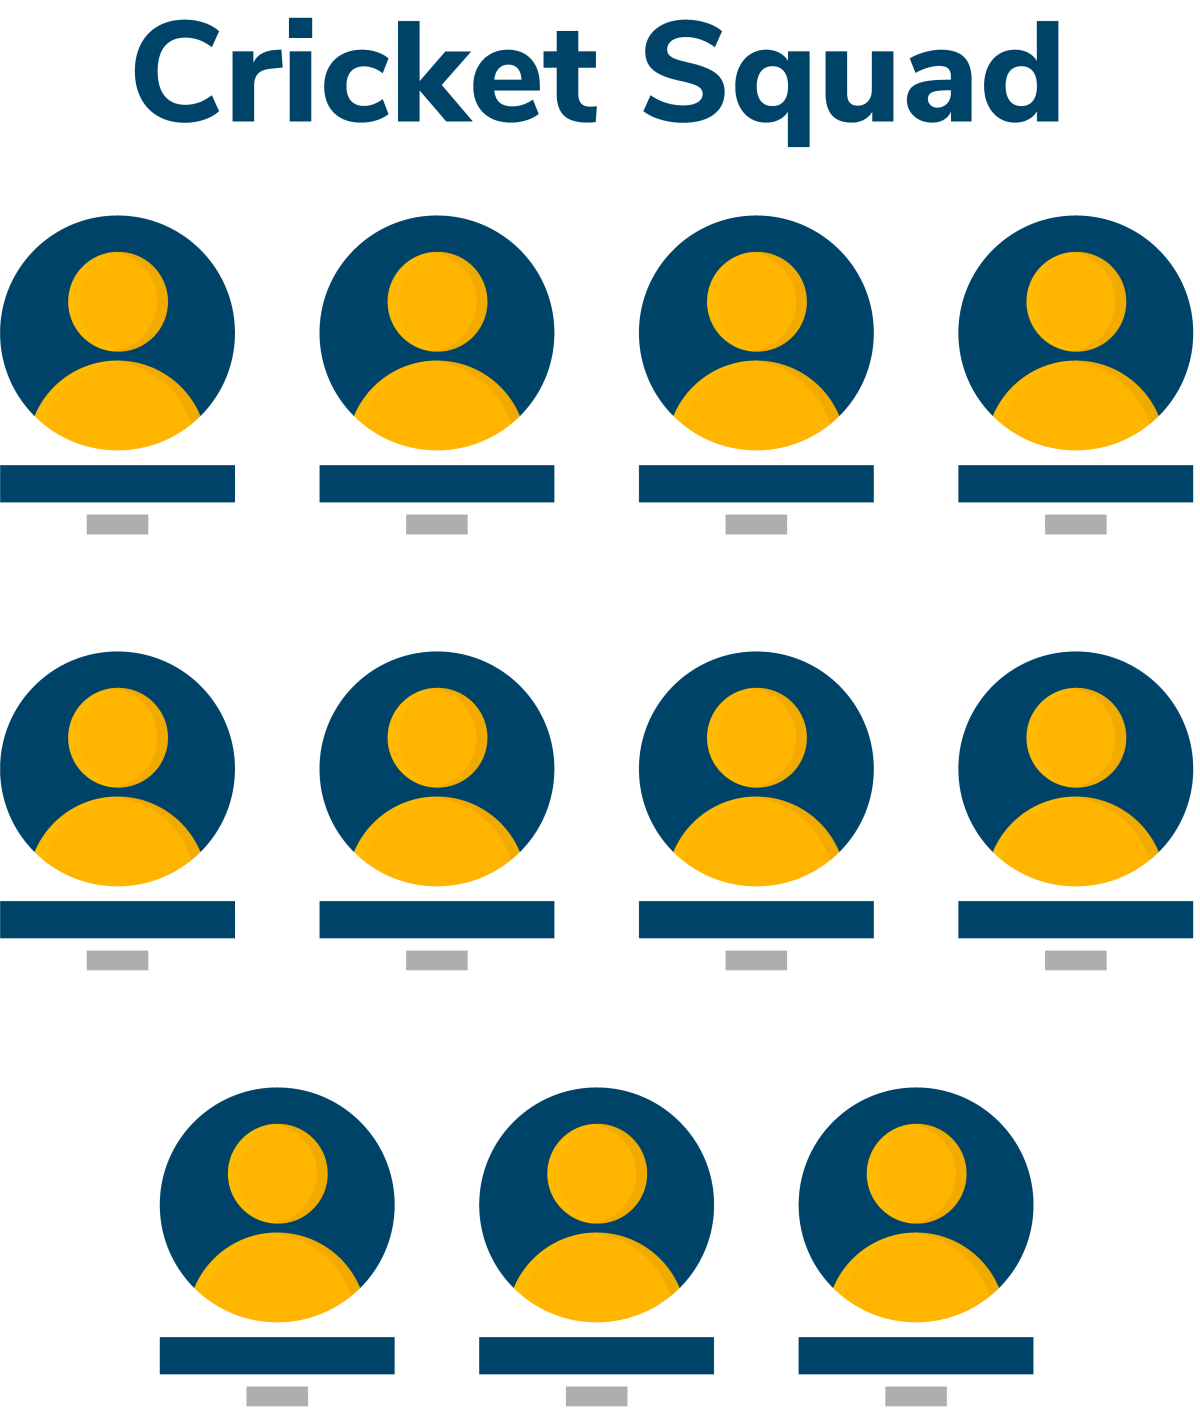
\includegraphics[width=0.5\textwidth]{Images/chapter_26/section_5684717988085760/5115267140288512.png}
\end{minipage}

We've identified our requirements for the problem. In the next lesson, we will define different use cases of ESPNcricinfo.

% End of section content